\documentclass[12pt,a4paper,UTF8]{ctexart}
\usepackage{geometry}
	\geometry{left=2.5cm,right=2.5cm,top=2cm,bottom=2cm}
\usepackage{xeCJK,amsmath,paralist,enumitem,booktabs,multirow,graphicx,subfig,setspace}
	\setlength{\parindent}{2em}
\usepackage[colorlinks,linkcolor=blue,urlcolor=blue]{hyperref}

%%%%%%%%%%%%%%%%%%%%%%%%%正文开始%%%%%%%%%%%%%%%%%%%%%%%%%%
\begin{document}

\title{\vspace{-2cm}\LARGE\bfseries C3.3 基于光纤光谱仪的吸收光谱测量\footnotemark[1]}
\author{\large\textit{黄子维}$^{1}$\footnotemark[2],\large\textit{黄睿杰}$^{2}$\footnotemark[3] \\ 
\small{1,2 \textit{中山大学 中山医学院,广东 广州 }510275}}
\date{}
\maketitle
\setcounter{page}{0}
\thispagestyle{empty}
\vspace{-1.5em}
\begin{spacing}{2.0}
{\bfseries 摘 {} 要:}
比尔-朗博定律指出,当光透过一定浓度溶液时,溶液中的吸光分子将吸收光,导致光强减弱。
当溶液浓度不大时,液体吸收系数与浓度成正比。这一理论揭示了溶液吸光规律,并且在利用吸收光谱分析法快速测定溶液浓度等领域有着重要应用。
本实验中,我们使用光纤光谱仪测量溴钨灯通过不同浓度红墨水溶液的吸收光谱,并计算吸收系数,验证比尔定律及其成立条件(如图\ref{fig:0})。

我们首先测量并比较了溴钨灯光谱、空比色皿吸收光谱与纯水吸收光谱,发现纯水在可见光范围内对光一般吸收,光谱峰值波长几乎不变,而空比色皿吸收光谱相对强度较弱。
接下来,我们测量了不同浓度红墨水溶液的吸收光谱,发现随浓度上升,吸收光谱峰值波长向长波方向移动。
最后我们计算了不同浓度红墨水溶液的吸收系数,发现在较低浓度,吸收系数与浓度成正比,但在较高浓度,溶液对光吸收趋于饱和。

\begin{figure}[htbp]
	\centering
	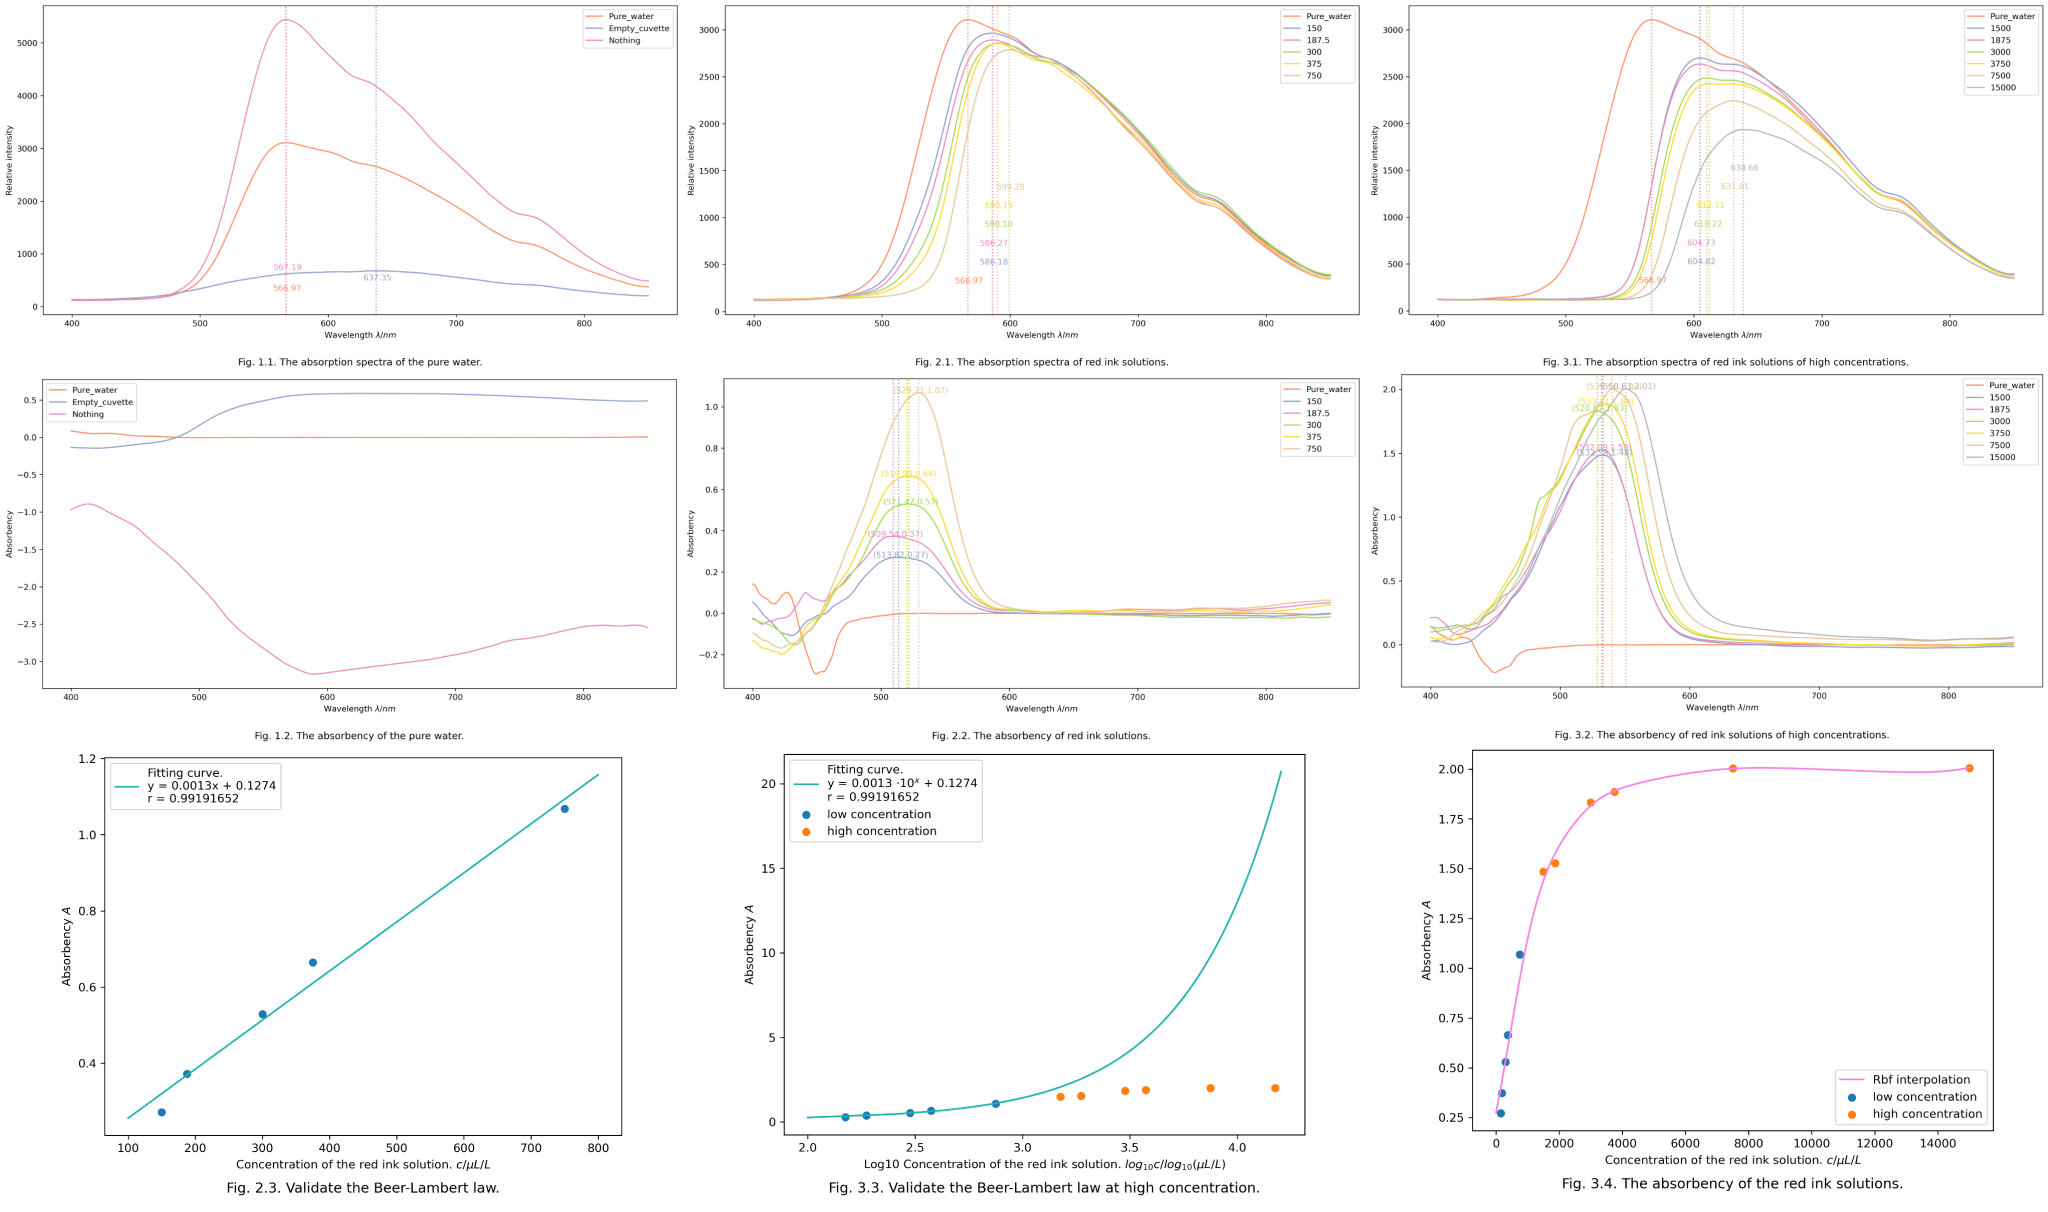
\includegraphics[width=0.8\textwidth]{attachments/Fig.0.pdf}
	\caption{不同浓度红墨水溶液吸收光谱及吸光度}
	\label{fig:0}
\end{figure}
\par
\vspace{-0.5em}
\bfseries{关键词}: 光纤光谱仪,吸收光谱,比尔-朗博定律
\vspace{0.5em}
\end{spacing}

\renewcommand{\thefootnote}{\fnsymbol{footnote}}
\footnotetext[1]{由中山大学物理学院陆佑堂提供器材和指导。}
\footnotetext[2]{通信作者,20980066,\url{huangzw29@mail2.sysu.edu.cn}}
\footnotetext[3]{实验参与人,20980062}

%%%%%%%%附录:数据处理%%%%%%%
\newpage
\pagestyle{plain}
\begin{center}
\LARGE\textbf{实验C3.3 基于光纤光谱仪的吸收光谱测量}
\end{center}

%%信息
\begin{doublespacing}
	\centering
	\begin{tabular}{ll}
	 & \\
	{\CJKfontspec{Droid Sans Fallback} 实验人:黄子维 20980066} & {\CJKfontspec{Droid Sans Fallback}合作者:黄睿杰 20980062}\\
	{\CJKfontspec{Droid Sans Fallback} 实验时间:2021.10.14~星期四~上午} & {\CJKfontspec{Droid Sans Fallback} 室温:24$^{\circ}$C~相对湿度:75\%}
	\end{tabular}
\end{doublespacing}
\subsection*{【实验参数】}
积分时间:1;平均次数:3;平滑宽度:2;波段:$400 \sim 850$;触发阈值:1000。

曲线平滑方法为径向基插值(Rbf),光滑度选取是经验的。

\subsection*{【数据处理及分析】}
\subsubsection*{1. 纯水吸收光谱}
使用光纤光谱仪分别测量光源溴钨灯光谱,空比色皿吸收光谱和纯水吸收光谱,结果如图\ref{fig:1.1}所示。
由吸收光谱计算吸收度如图\ref{fig:1.2}所示(以纯水吸收为标准参考,下同)。

\begin{figure}[htbp]
	\centering
	\subfloat[吸收光谱]{\label{fig:1.1}
	\includegraphics[width=0.45\textwidth]{attachments/Fig.1.1.png}
	}
	\subfloat[吸收度]{\label{fig:1.2}
	\includegraphics[width=0.45\textwidth]{attachments/Fig.1.2.png}
	}
	\caption{纯水吸收光谱和吸收度}
\end{figure}
	
观察图\ref{fig:1.1},发现纯水在可见光范围内对光一般吸收,光谱峰值波长$(566.97 nm)$相对溴钨灯光谱峰值波长$(567.19 nm)$几乎不变。而空比色皿吸收光谱相对强度较弱,光谱峰值波长更大$(637.35 nm)$。
将纯水吸收光谱定为标准参考,如图\ref{fig:1.2},此时纯水吸收度几乎为$0$,说明标定有效。

\subsubsection*{2. 低浓度红墨水溶液吸收光谱及吸光度规律}
使用光纤光谱仪分别测量低浓度下不同浓度红墨水溶液吸收光谱,结果如图\ref{fig:2.1}所示。
各浓度溶液吸收光谱峰值波长如表\ref{tab:2.1},发现随红墨水溶液浓度上升,吸收光谱峰值波长向长波方向移动。

由吸收光谱计算不同浓度红墨水溶液吸收度,如图\ref{fig:2.2}所示。
吸收度峰值波长及对应吸收度如表\ref{tab:2.2},发现随红墨水溶液浓度上升,吸收度峰值波长也大致遵循向长波方向移动的规律,且峰值吸收度不断增大。

取各浓度下峰值吸收度,绘制吸收度随浓度变化关系,发现在较低浓度范围内二者成正比(如图\ref{fig:2.3})。直线拟合方程$y = 0.0013x+0.1274$,相关系数$r = 0.99$。
这就验证了低浓度溶液吸光度遵循比尔定律。                                            
\begin{figure}[htbp]
	\centering
	\subfloat[吸收光谱]{\label{fig:2.1}
	\includegraphics[width=0.45\textwidth]{attachments/Fig.2.1.png}
	}
	\subfloat[吸收度]{\label{fig:2.2}
	\includegraphics[width=0.45\textwidth]{attachments/Fig.2.2.png}
	}
	\caption{低浓度红墨水溶液吸收光谱和吸收度}
\end{figure}

\begin{table}[htbp]
	\centering
	\begin{minipage}{0.45\linewidth}
		\begin{tabular}{cc}
			\toprule
			浓度$c(\mu L/L)$ &峰值波长$\lambda (nm)$ \\
			\midrule
			0 &566.97 \\		
			150 &586.18 \\
			187.5 &586.27 \\
			300 &590.10 \\
			375 &590.19 \\
			700 &599.28 \\
			\bottomrule
		\end{tabular}
		\caption{\textbf{低浓度溶液吸收光谱峰值波长}}
		\label{tab:2.1}
	\end{minipage}
	\begin{minipage}{0.45\linewidth}
		\begin{tabular}{ccc}
			\toprule
			浓度$c(\mu L/L)$ &峰值波长$\lambda (nm)$ &峰值吸收度 \\
			\midrule
			0 &/ &0 \\		
			150 &513.82 &0.27 \\
			187.5 &509.54 &0.37 \\
			300 &521.47 &0.53 \\
			375 &519.98 &0.66 \\
			700 &529.21 &1.07 \\
			\bottomrule
		\end{tabular}
		\caption{\textbf{低浓度溶液峰值吸收度}}
		\label{tab:2.2}
	\end{minipage}
\end{table}

\begin{figure}[htbp]
	\centering
	\includegraphics[width=0.4\textwidth]{attachments//Fig.2.3.png}
	\caption{验证比尔定律}
	\label{fig:2.3}
\end{figure}


\subsubsection*{3. 高浓度红墨水溶液吸收光谱及吸光度规律}
使用光纤光谱仪分别测量高浓度下不同浓度红墨水溶液吸收光谱,结果如图\ref{fig:3.1}所示。
各浓度溶液吸收光谱峰值波长如表\ref{tab:3.1},发现随红墨水溶液浓度上升,吸收光谱峰值波长向长波方向移动。

由吸收光谱计算不同浓度红墨水溶液吸收度,如图\ref{fig:3.2}所示。
吸收度峰值波长及对应吸收度如表\ref{tab:3.2},发现随红墨水溶液浓度上升,吸收度峰值波长也大致遵循向长波方向移动的规律,且峰值吸收度不断增大。

取各浓度下峰值吸收度,绘制吸收度随浓度变化关系,发现在高浓度范围内,溶液吸光度不再遵循比尔定律。
如图\ref{fig:3.3},横坐标为对数浓度,曲线为比尔定律曲线,发现高浓度溶液吸光度(橙色)明显偏离比尔定律预测值。
如图\ref{fig:3.4},曲线为径向基插值拟合,发现在溶液浓度$6000 \mu L/L$附近溶液吸光度趋近饱和。                                                      
\begin{figure}[htbp]
	\centering
	\subfloat[吸收光谱]{\label{fig:3.1}
	\includegraphics[width=0.45\textwidth]{attachments/Fig.3.1.png}
	}
	\subfloat[吸收度]{\label{fig:3.2}
	\includegraphics[width=0.45\textwidth]{attachments/Fig.3.2.png}
	}
	\caption{高浓度红墨水溶液吸收光谱和吸收度}
\end{figure}

\begin{table}[htbp]
	\centering
	\begin{minipage}{0.45\linewidth}
		\begin{tabular}{cc}
			\toprule
			浓度$c(\mu L/L)$ &峰值波长$\lambda (nm)$ \\
			\midrule
			0 &566.97 \\		
			1500 &604.82 \\
			1875 &604.73 \\
			3000 &610.22 \\
			3750 &612.11 \\
			7500 &631.01 \\
			15000 &638.66 \\
			\bottomrule
		\end{tabular}
		\caption{\textbf{高浓度溶液吸收光谱峰值波长}}
		\label{tab:3.1}
	\end{minipage}
	\begin{minipage}{0.45\linewidth}
		\begin{tabular}{ccc}
			\toprule
			浓度$c(\mu L/L)$ &峰值波长$\lambda (nm)$ &峰值吸收度 \\
			\midrule
			0 &/ &0 \\		
			1500 &532.58 &1.48 \\
			1875 &532.09 &1.53 \\
			3000 &528.67 &1.83 \\
			3750 &533.71 &1.89 \\
			7500 &539.96 &2.00 \\
			15000 &550.63 &2.01 \\
			\bottomrule
		\end{tabular}
		\caption{\textbf{高浓度溶液峰值吸收度}}
		\label{tab:3.2}
	\end{minipage}
\end{table}

\begin{figure}[htbp]
	\centering
	\subfloat[验证高浓度溶液是否符合比尔定律]{\label{fig:3.3}
	\includegraphics[width=0.35\textwidth]{attachments/Fig.3.3.png}
	}
	\subfloat[吸光度与溶液浓度的关系]{\label{fig:3.4}
	\includegraphics[width=0.35\textwidth]{attachments/Fig.3.4.png}
	}
	\caption{验证比尔定律成立条件}
\end{figure}

\newpage
\subsection*{【思考题】}
\subsubsection*{1. 根据红墨水吸收峰波长,如何选择光源,理由?}
答:应选择发射波段在吸收峰附近波段内的光源。红墨水吸收峰波长大致为$550nm \sim 650nm$,
结合实验C3.1,溴钨灯光源在该波段发射光谱强度较强,选择溴钨灯为光源容易在吸收光谱上观察到吸收峰的现象。
\subsubsection*{2. 比较发射光谱和吸收光谱光路设置异同。}
答:发射光谱采用光学多道分析仪,吸收光谱采用光纤光谱仪。两者部分光路相同,都由光线从入射狭缝射入,经准光镜反射至光栅,实现分光。
不同之处在于光学多道分析仪采用物镜将光栅出射光线聚焦到出射狭缝,由感光元件测量光信号。这一过程由步进电机控制,使每一时刻感光元件采集到的光信号为特定波长的光。
而光纤光谱仪采用聚焦镜将光栅出射光线投射到探测器聚光透镜,再由探测器检测光信号,每一时刻探测器可同时测量量程范围所有波长光的光强。
\subsubsection*{3. 比较光栅光谱仪和光纤光谱仪优缺点,试举排他例子。}
答:光栅光谱仪的分辨率高,但设备不便于携带,且内部结构精细,使用需要标定和精密调节。同时光栅光谱仪只能逐波长扫描,测量速度慢;
光纤光谱仪的灵敏度较高,且体积较小,使用环境要求不高,便于便携使用,同时光纤光谱仪可以实现即时测量,快速获得光谱,但分辨率可能不够。
精密测量实验,如测量原子发射光谱,特别是例如钠双黄线测量,就需要使用光栅光谱仪。
而需要快速测量光谱的实验,如动态监测光谱变化,就需要使用光纤光谱仪。
\subsection*{【项目源码】}
\href{https://github.com/Jeg-Vet/SYSU-PHY-EXP/tree/main/C3.3-Absorption_spectra}{SYSU-PHY-EXP/C3.3 Absorption spectra @Jeg-Vet(github.com)}

\end{document}

